% !TeX root = thesis.tex
\chapter{Data}

This thesis uses two data sources. LINCS L1000 gene expression data show how cells respond to drug treatment. The OmniPath interaction database gives known information about how genes and proteins are linked. LINCS provides the drug response data, while OmniPath provides the graph used by the graph based models.
\noindent Unless otherwise stated, figures from this chapter were created by the author.

\section{CMap LINCS Dataset}
The NIH Common Fund’s Library of Integrated Network based Cellular Signatures (LINCS) provides large datasets for studying how cells respond to chemical and genetic changes. A major part of LINCS is the L1000 assay~\cite{l1000_paper}. The assay directly measures the expression of 978 landmark genes~\cite{l1000_paper}. These genes were chosen because they capture a large part of the change in gene expression across many biological conditions. The L1000 pipeline can also estimate additional genes from the measured landmark genes, which gives a wider gene space of 12,328 genes in total. The data are widely used because they cover many compounds, cell lines, and experimental conditions, together with matched control samples.

\noindent Public LINCS L1000 data have been released through resources such as the GEO archive and later combined releases including CMap LINCS 2020. The present work uses these public releases as the main source of perturbation expression data.
\noindent The LINCS L1000 data used in this thesis include control expression data, treatment expression data, metadata, and drug annotation information. Control expression data describe the baseline state of cells without the active drug. Treatment expression data describe gene expression after drug exposure. Metadata record the experimental background, such as cell line, dose, treatment time, and plate related information. Drug annotation information provides compound identifiers, reported targets, and related compound descriptions.


\subsection{L1000 Data Processing Flow}
In these public resources, the data are commonly organized into several processing levels for the same experiments:
\begin{enumerate}
\item \textbf{Level 1: Raw measurement values.} These are the original values recorded in the experiment.
\item \textbf{Level 2: Gene expression values.} The raw values are converted into gene expression values.
\item \textbf{Level 3: Normalized expression data.} The data are adjusted so that samples can be compared more fairly. At this level, expression for genes beyond the 978 landmark genes is also estimated.
\item \textbf{Level 4: Drug effect profiles.} Treatment samples are compared with matched control samples to show how the drug changes gene expression.
\item \textbf{Level 5: Combined summary profiles.} Repeated measurements are combined into one more stable summary result.
\end{enumerate}

\noindent This thesis uses the normalized and inferred gene expression matrix from Level 3. Figure~\ref{fig:data_level} shows the full processing flow. These data provide normalized and inferred gene expression profiles in a common gene space across samples.

\noindent Level 3 is used because this project needs the treated expression profile and the matched control profile as two separate inputs. The response target is constructed later from these two profiles inside the present pipeline. This is also important because the matched control profile is used as a model input and as the source of cell context. Level 2 is less suitable because it is an earlier processing stage and does not yet provide the normalized expression profiles used for reliable comparison across samples. It also does not provide the inferred wider gene space used in the standard Level 3 release. Level 4 is less suitable for this design because it already stores the result after treatment and control have been compared. In other words, it is no longer the original treated profile and the original control profile stored side by side in the same simple form. That makes it harder to use the matched control directly as an input to the model. Level 5 is even further from the present task, because it combines repeated measurements into one summary result. That is useful for some analyses, but it removes sample specific variation that is needed here for paired prediction and uncertainty analysis.

\begin{figure}[htbp]
    \centering
    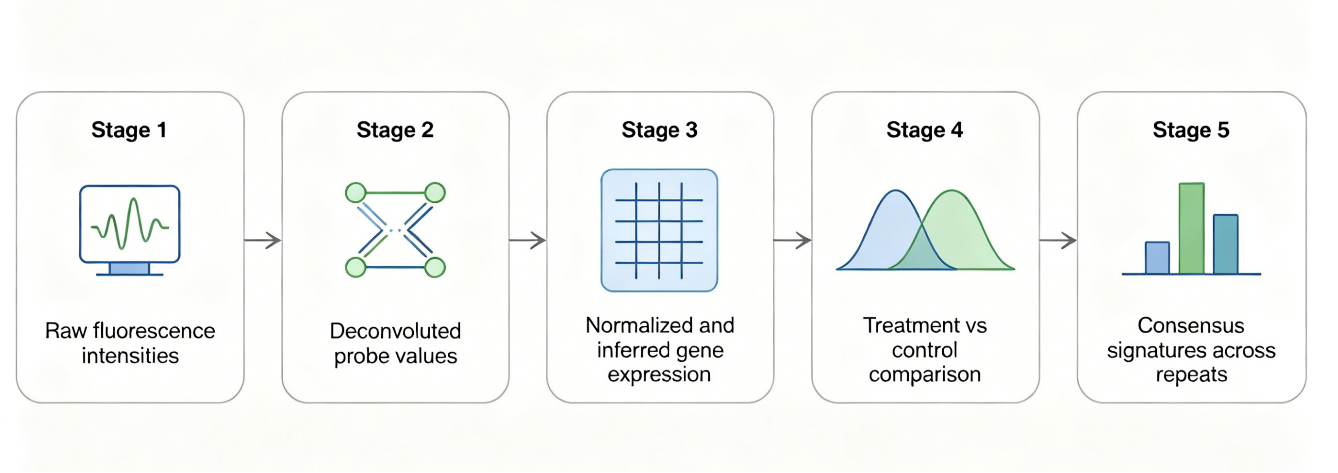
\includegraphics[width=0.95\linewidth]{figures/data_level.png}
    \caption[LINCS Processing Workflow]{LINCS L1000 data processing workflow. The pipeline moves from raw measurement values in Level 1 to gene expression values in Level 2, normalized expression data in Level 3, drug effect profiles in Level 4, and combined summary profiles in Level 5. Created by the author with AI assistance.}
    \label{fig:data_level}
\end{figure}


\subsection{Treatment and control data}
\noindent LINCS experiments include both compound treatment profiles and matched control profiles. In the control condition, cells receive the same DMSO vehicle as the drug treatment, but no active compound. These profiles cover many cell lines, compounds, and experimental conditions, and each profile is stored as a gene expression vector in the shared gene space. Treatment profiles describe the cell state after drug exposure, whereas control profiles describe the corresponding setting without the active drug.

\subsection{Metadata}
\noindent Metadata come from the LINCS annotation table that is released with the Level 3 expression data~\cite{l1000_paper}. Each row describes one perturbation record. The table includes compound identity, cell line, experimental conditions, quality control, and batch related variables. These fields give the biological and technical context for the expression matrices. Reliable pairing, filtering, grouping, and evaluation depend on this information.

\noindent The metadata also record the experimental condition through fields such as \texttt{pert\_dose}, \texttt{pert\_dose\_unit}, \texttt{pert\_time}, and \texttt{pert\_time\_unit}. In addition, they include technical context variables such as \texttt{bead\_batch}, \texttt{det\_plates}, and \texttt{det\_wells}. These fields are useful because two samples may look different for technical reasons even when their biology is similar. Without this information, treatment and control samples could be matched across different technical conditions.

\noindent Quality control is also described in the metadata~\cite{l1000_paper}. Some records are weak or noisy, so the table includes fields such as \texttt{is\_hiq} and \texttt{qc\_pass}. Other summary fields, such as \texttt{tas}, describe how strong and reproducible the measured response is. These variables help identify more reliable profiles and remove noisier ones.


\subsection{Drug target}
\noindent Drug related information is collected from the compound annotation table. It stores compound names in \texttt{cmap\_name}, target annotations in \texttt{target}, and mechanism of action descriptions in \texttt{moa}. In this thesis, it is used to identify which genes are reported as targets of each drug, so that drug specific input signals can be matched to the expression matrix and the OmniPath graph.

\noindent The \texttt{target} field lists reported protein or gene targets for a subset of compounds. One drug may have several targets, so the field can contain more than one gene. During preprocessing, these target names are mapped to the gene identifiers used in the selected expression space. Only targets that align with the expression matrix and the graph can be used by the model. Target information is not available for all compounds in LINCS because many compounds are still not fully characterized.

% \paragraph{Molecular fingerprints.}
% To reduce reliance on incomplete target annotations, we also use molecular fingerprints (for example, Morgan/ECFP) as a fixed length representation of chemical structure. Fingerprints provide dense drug features even when curated target annotations are missing, and they support generalization across compounds based on structural similarity.

\subsection{Table association}
\noindent The main tables are linked by shared identifiers. This makes it possible to trace each expression profile back to its experimental context, including cell line, dose, time, batch, and plate information, and to its compound annotation. These links support consistent filtering, grouping, and matched treatment control comparisons.

\noindent Table~\ref{tab:lincs_key_fields} lists the main identifiers and quality related variables that appear in this chapter. They belong to four simple groups: sample identifiers, experimental condition fields, technical batch fields, and quality control fields.

\begin{table}[htbp]
    \centering
    \caption[Main LINCS Fields]{Main LINCS fields used in this chapter. The table gives a short meaning for each field and shows which table it comes from.}
    \label{tab:lincs_key_fields}
    \begin{tabular}{>{\raggedright\arraybackslash}p{2.2cm}>{\raggedright\arraybackslash}p{7.1cm}>{\raggedright\arraybackslash}p{3.0cm}}
        \hline
        Field & Meaning & Source table \\
        \hline
        \texttt{distil\_id} & One expression profile identifier. It points to one row in the Level 3 expression matrix. & Level 3 expression matrix \\
        \texttt{distil\_ids} & One or more \texttt{distil\_id} values linked to the same metadata record. & meta table \\
        \texttt{sig\_id} & Unique identifier for one perturbation record. & meta table \\
        \texttt{pert\_id} & Compound identifier used to link metadata records to compound annotations. & meta table, compound annotation table \\
        \texttt{bead\_batch} & Identifier for the technical bead batch used in the assay. & meta table \\
        \texttt{det\_plates} & Identifier for the detection plate used in the measurement process. & meta table \\
        \texttt{is\_hiq} & Simple high quality flag for a metadata record. & meta table \\
        \texttt{qc\_pass} & Flag that shows whether a metadata record passed quality control. & meta table \\
        \texttt{tas} & Summary score that reflects response strength and reproducibility. & meta table \\
        \hline
    \end{tabular}
\end{table}

\noindent Level 3 expression matrices are indexed by \texttt{distil\_id}. The metadata table contains \texttt{distil\_ids}, which stores one or more \texttt{distil\_id} values for each metadata record. This field links metadata to expression profiles. Each metadata row also contains a unique record identifier \texttt{sig\_id}, a compound identifier \texttt{pert\_id}, and a cell line name \texttt{cell\_iname}. The compound annotation table uses \texttt{pert\_id} as its primary key, which links metadata records to drug target annotations.


% \textbf{Molecular fingerprints} provide a fixed length representation of a compound's chemical structure by encoding the presence of local substructures (for example, Morgan or ECFP fingerprints). Fingerprints allow the model to compare drugs based on structural similarity even when target annotations are incomplete. Both feature types are linked to expression profiles through the compound identifier.

% \begin{figure}[htbp]
%     \centering
%     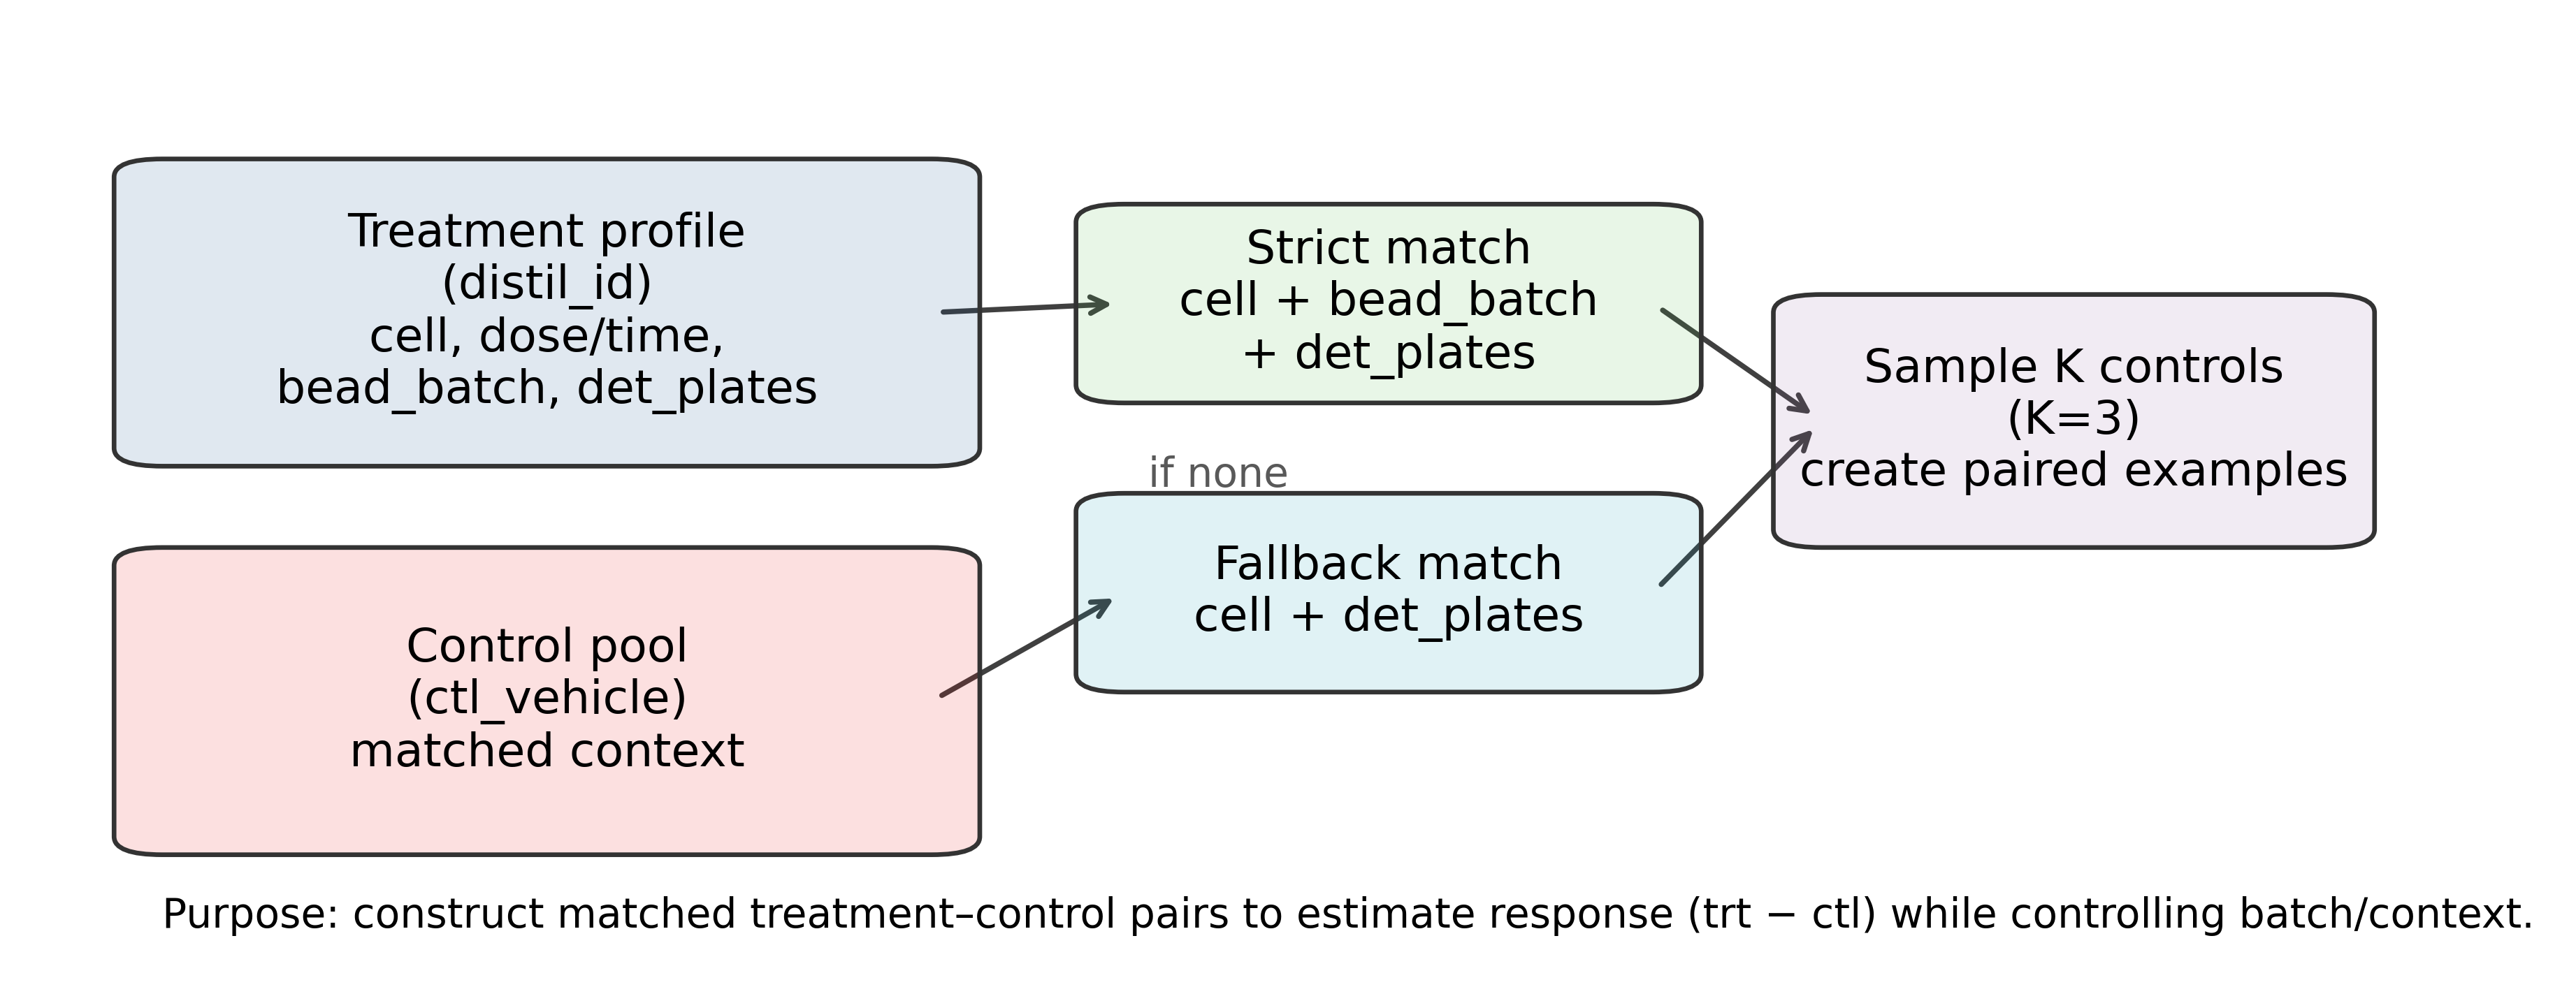
\includegraphics[width=0.95\linewidth]{figures/paired_construction_schematic.png}
%     \caption{Schematic of paired sample construction. Treatment profiles are matched to vehicle controls using strict and relaxed context rules, and multiple matched controls can be sampled for the same treatment profile to form paired modelling examples.}
%     \label{fig:paired_construction_schematic}
% \end{figure}

\FloatBarrier
\section{OmniPath Dataset}
\noindent OmniPath is a public database of gene and protein interactions in human cells~\cite{turei2016omnipath}. It collects control related information from many studies and databases. This thesis uses the regulatory subset of OmniPath. Each row describes a regulator protein, its target gene, and whether the reported effect is activating or inhibiting.

\noindent For each interaction, OmniPath stores fields that describe direction, sign, and evidence. For example, \texttt{is\_directed}, \texttt{is\_stimulation}, and \texttt{is\_inhibition} indicate whether the interaction is directed and whether it is activating or inhibiting. Evidence related fields such as \texttt{sources}, \texttt{n\_sources}, \texttt{n\_primary\_sources}, and \texttt{n\_references} summarize how many databases and publications support an interaction.

\noindent OmniPath combines interactions from many sources, so different sources may report different labels for the same edge. One source may report stimulation, while another may report inhibition. OmniPath stores both individual labels and combined fields. These fields can be used during graph construction.

\noindent Genes from the LINCS expression matrix are mapped to nodes in the OmniPath regulon graph. The resulting directed network encodes transcription factor to gene relationships that are supported by published studies. When this network is combined with gene expression data, the model can use both measured responses and known control information.

\FloatBarrier
\section{Data preprocessing}

\noindent The LINCS Level 3 matrices and metadata are preprocessed so that suitable samples can be filtered, matched treatment and control profiles can be constructed, and the final data can be organized into a form that the GNN can learn from.

\subsection{CMap LINCS L1000 preprocessing}

\subsubsection{Gene set selection}
Two gene spaces are supported. In landmark mode, the 978 landmark genes are used in the order given by the landmark gene list. In full gene mode, all 12,328 genes are loaded from the LINCS gene information table and \texttt{pr\_gene\_id} is used as the identifier. In both cases, one fixed gene order is used across control profiles, treatment profiles, response targets, and drug vectors. This keeps all matrices aligned.

\subsubsection{Metadata filtering}
Preprocessing starts from the metadata table. Figure~\ref{fig:l1000_filter_flow} summarizes the effect of the main filtering steps. To reduce heterogeneity across experiments, one fixed condition is used throughout this work, namely 24 h and 10 \textmu M. This practical choice keeps samples more comparable while still allowing measurable gene expression responses after treatment. High quality treatment profiles are also retained through the quality flags in the metadata.
\begin{figure}[htbp]
    \centering
    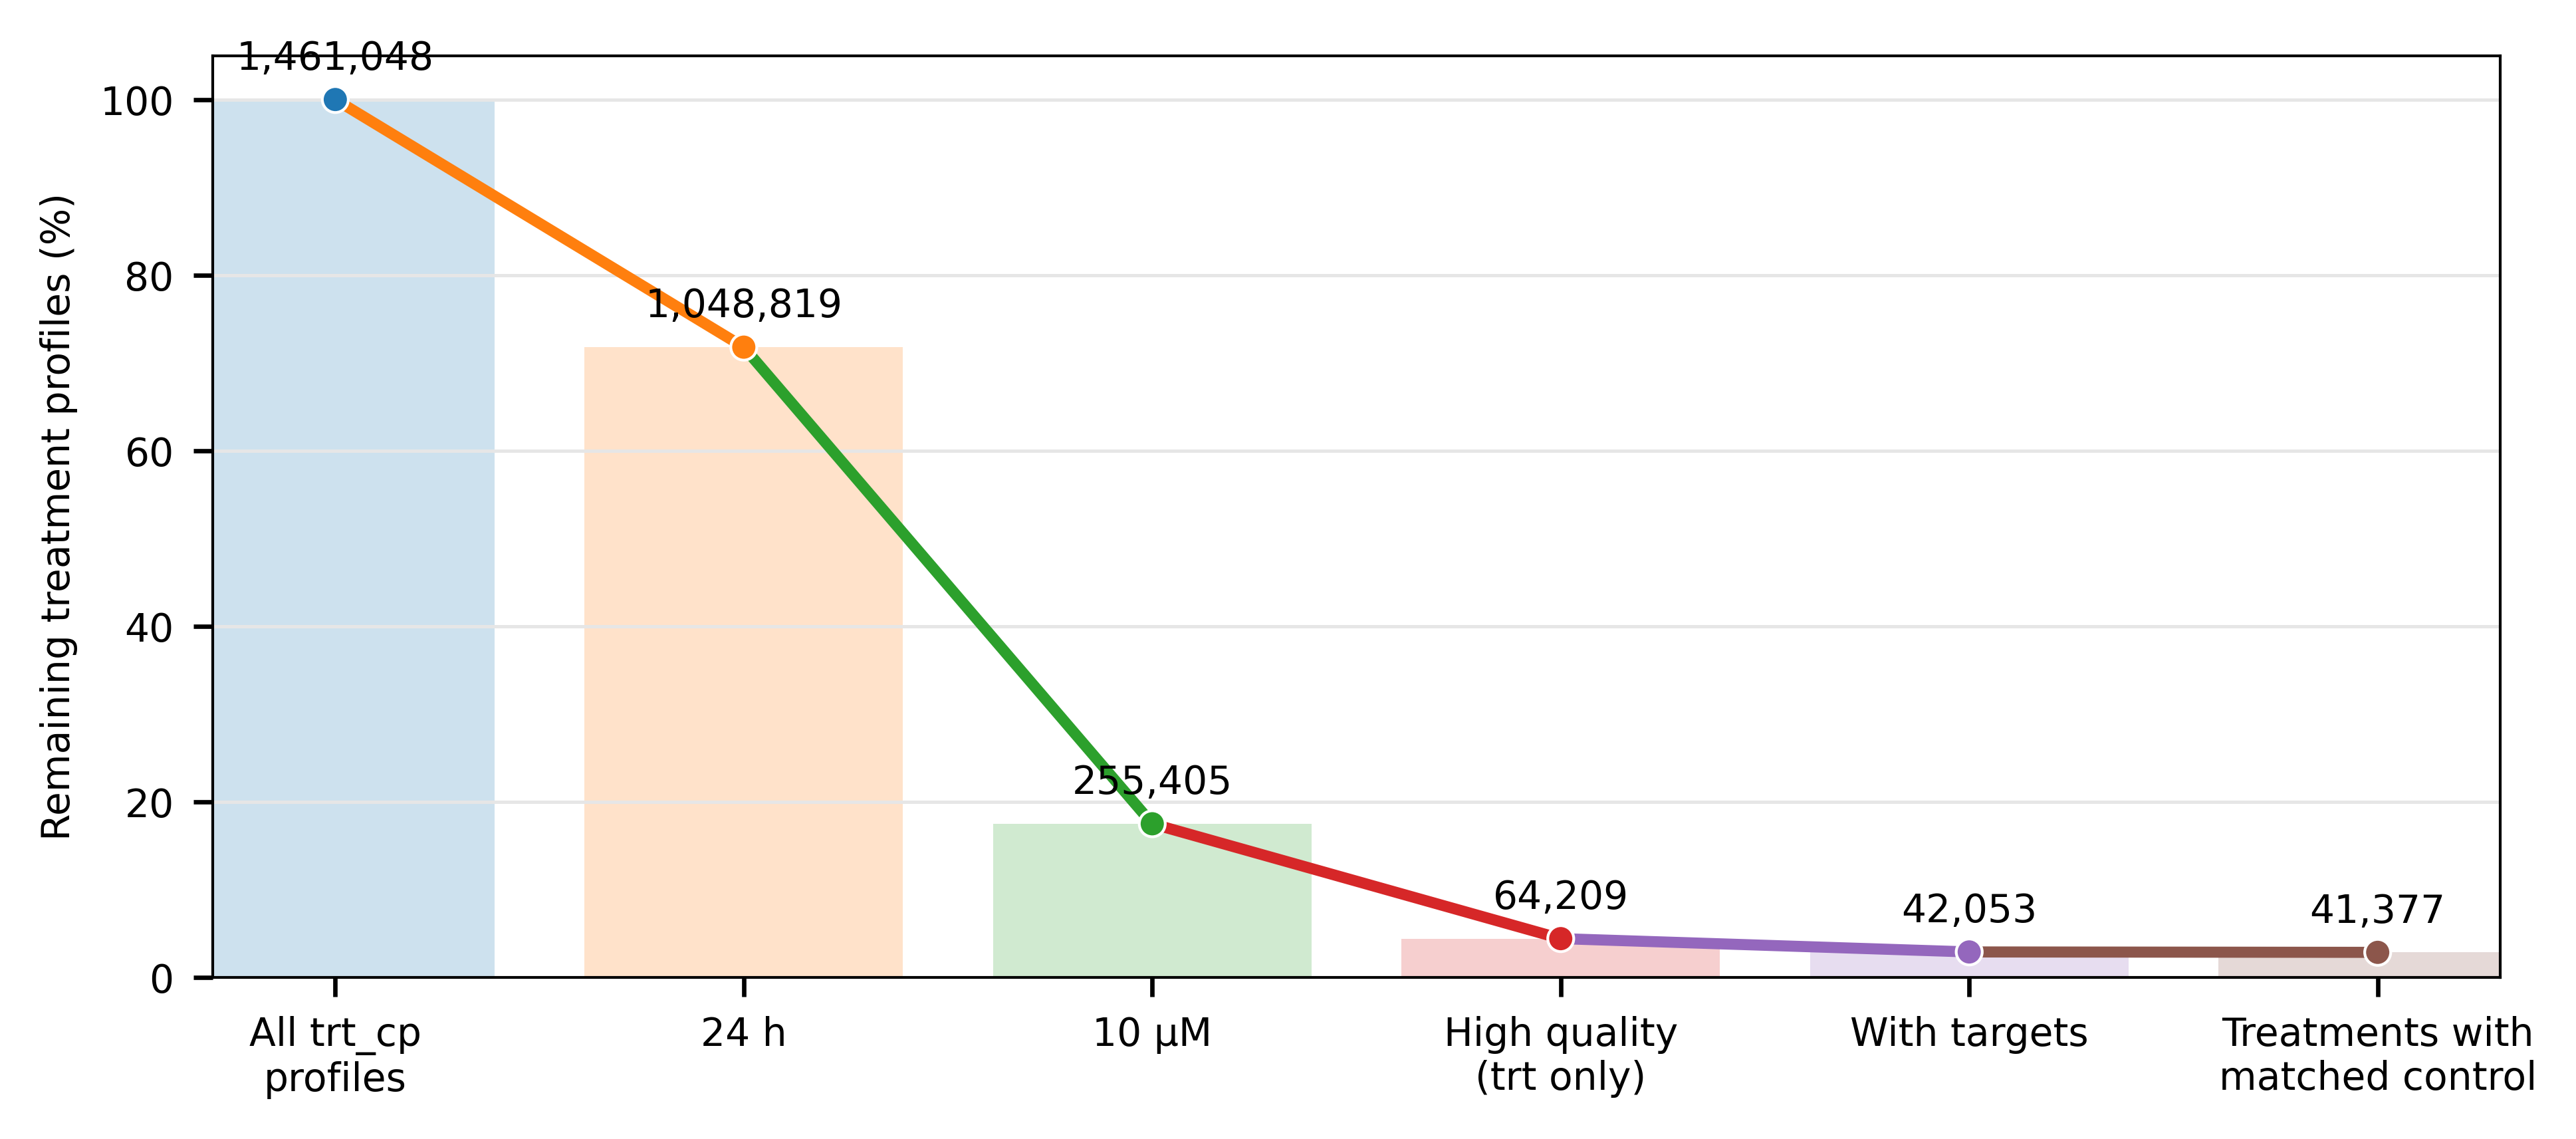
\includegraphics[width=0.95\linewidth]{figures/l1000_filter_flow.png}
    \caption[Treatment Profile Filtering]{Effect of successive filtering steps on the number of treatment profiles retained for modelling in a single dose and single time point setting. The final step counts treatment profiles that can be paired with at least one matched control sample that receives the same solvent but no active compound under the context matching rules.}
    \label{fig:l1000_filter_flow}
\end{figure}
\subsubsection{Treatment and control data filtering}
\noindent From the filtered metadata, control profiles are collected and the \texttt{distil\_ids} field is expanded so that each profile has one unique identifier. For each control profile, the cell line, bead batch, and detection plate are recorded. The expression vectors for these identifiers are then loaded from the Level 3 matrix. The loader reads only the requested identifiers and only the selected gene columns.

\noindent The same procedure is applied to treatment profiles. The field \texttt{distil\_ids} is expanded for each treatment record, and the cell line, compound identifier, bead batch, and detection plate are stored for each sample. The expression vectors for these treatment identifiers are then loaded from the Level 3 matrix.
\subsubsection{Random matching}
\noindent Each treatment profile is paired with matched control profiles so that the model learns the change caused by drug treatment rather than the full baseline state of the cell. This also helps reduce some shared technical variation when treatment and control are measured under similar conditions.

\noindent Control candidates are selected from the same cell line and the same experimental context. The primary rule matches cell line, bead batch, and detection plate. If no control is available under this exact rule, a relaxed rule matches cell line and detection plate. Treatment profiles without a suitable control are removed. After this step, each treatment profile is stored together with its candidate controls.

\noindent Final matching is carried out after the data split. Random matching is then applied within each split. In training, one treatment profile can be paired with several randomly sampled controls. If the candidate pool is smaller than the requested number of matches, sampling is done with replacement. In the test set, each treatment profile is paired with one control only. The supervised target is then constructed from the treatment expression vector $x_{\mathrm{trt}}$ and the matched control expression vector $x_{\mathrm{ctl}}$.

\subsubsection{Data leakage}
\noindent Several steps are used to reduce the risk of data leakage. Treatment profiles are split before the final treatment control pairs are sampled, and the control pools for training and test are kept separate. This prevents paired examples derived from the same treatment profile from appearing on both sides of the evaluation, and it also prevents the same control profile from being reused across training and test. In the cold drug target setting, test drugs are removed from training. In the cold cell setting, test cell lines are removed from training.

% \begin{figure}[htbp]
%     \centering
%     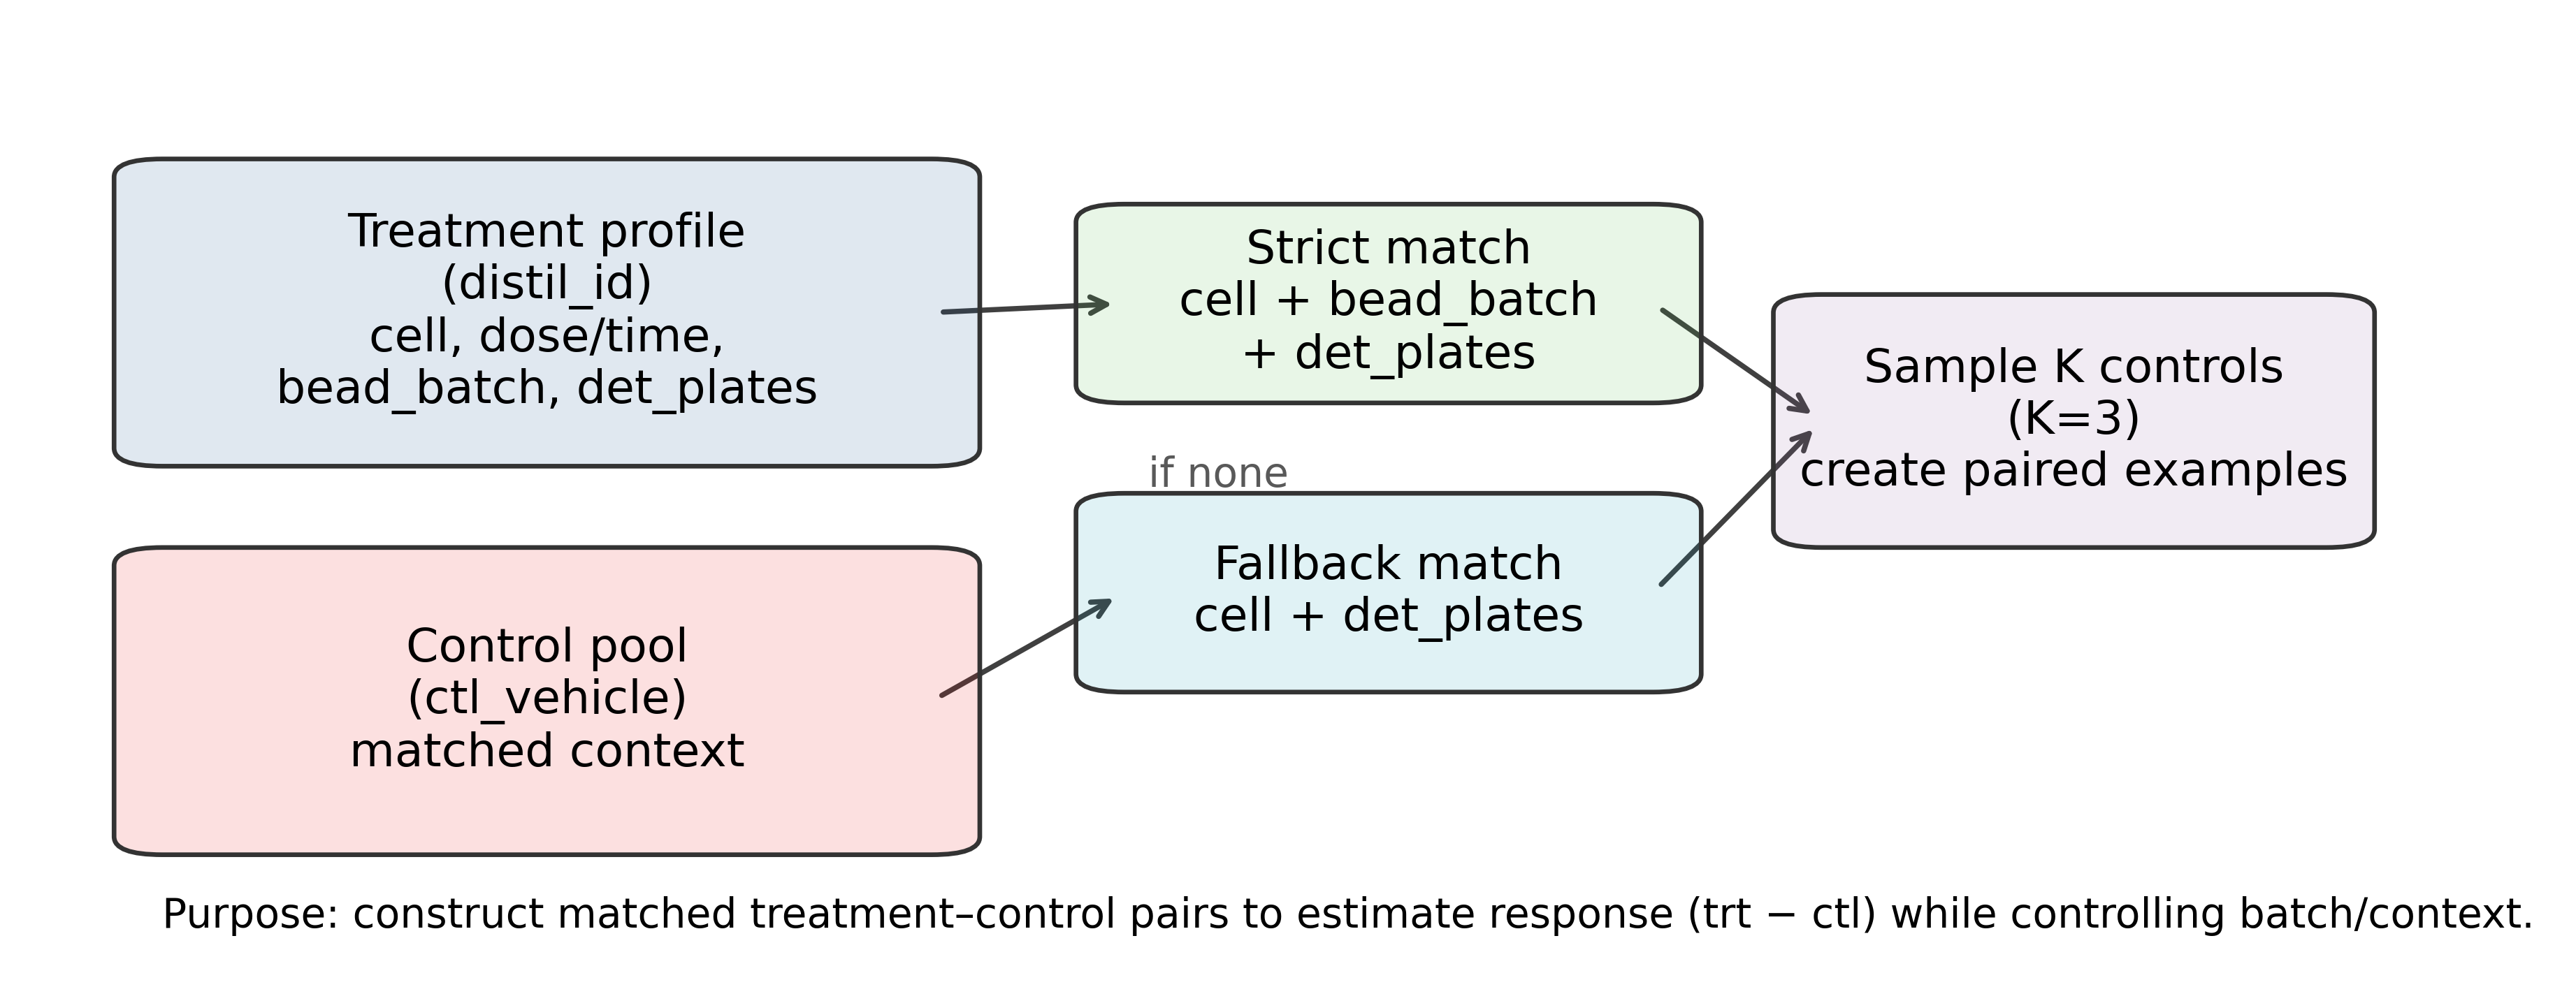
\includegraphics[width=0.95\linewidth]{figures/paired_construction_schematic.png}
%     \caption{Schematic of paired sample construction. Treatment profiles are matched to vehicle controls using strict and relaxed context rules, then multiple controls are sampled to form paired training examples.}
%     \label{fig:paired_construction_schematic}
% \end{figure}


\subsubsection{Drug filtering}
\noindent Every training example is linked to a compound identifier and for each drug, we build a target vector over the selected genes. If a gene is an annotated target of the drug, its position in the vector is marked; otherwise it remains zero. Only treatment examples with usable drug target annotations are retained in settings that require target based features. Examples whose \texttt{pert\_id} cannot be linked to an existing \texttt{target} field are removed.


% \begin{figure}[htbp]
%     \centering
%     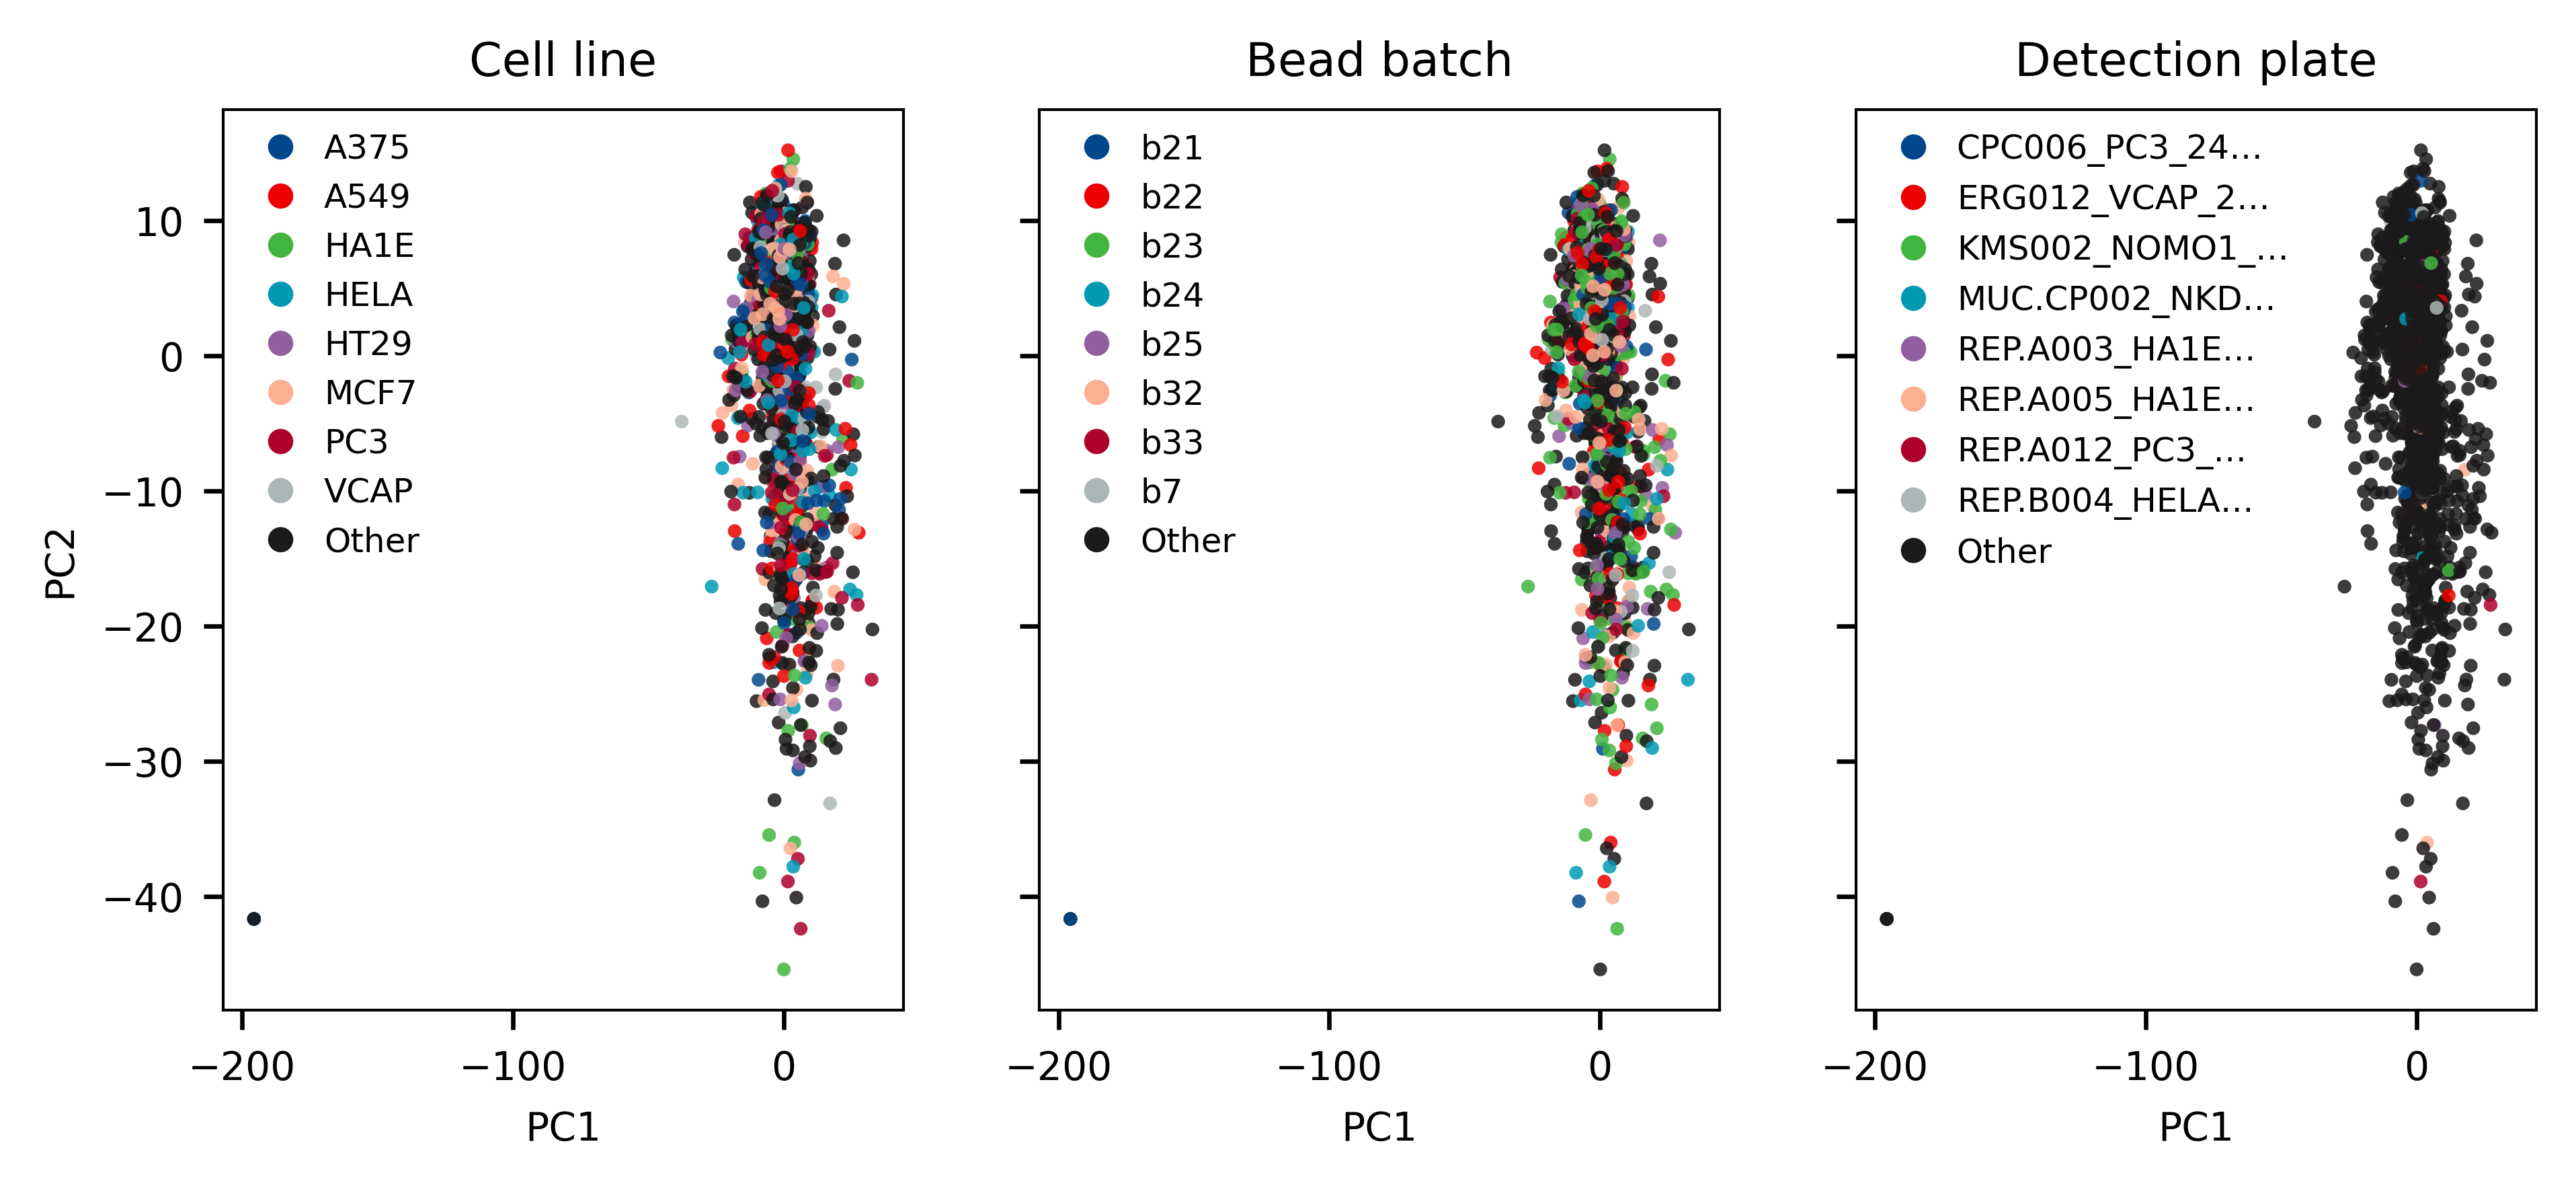
\includegraphics[width=0.95\linewidth]{figures/l1000_batch_pca.png}
%     \caption{PCA of control profiles (24\,h) in the 978 landmark gene space, coloured by cell line and technical factors. Visible structure indicates that batch and plate variables can contribute systematic variation and motivates matched pairing.}
%     \label{fig:l1000_batch_pca}
% \end{figure}

\subsection{OmniPath graph preprocessing}
\noindent The interaction graph is constructed from OmniPath resources that provide directed control or interaction links. The resulting graph is matched to the selected gene space. Each row describes a source gene and a target gene together with sign information when available.

\noindent OmniPath tables are provided in gene symbols. These symbols are mapped to the gene identifiers used by the expression matrices. Edges are kept only when both endpoints can be mapped and both genes are present in the selected gene set. This ensures that graph nodes, expression vectors, and drug target vectors all refer to the same ordered gene list.

\noindent The graph is represented as a directed edge list. When OmniPath provides sign annotations, each edge is assigned a sign value $w\in\{+1,-1\}$ for stimulation or inhibition. If sign information is missing, the edge can be excluded or treated as unknown, depending on the experiment setting.

\noindent An interaction may appear multiple times across sources. Duplicate edges are merged so that each ordered pair $(u,v)$ appears once in the final graph. The resulting graph is stored as \texttt{edge\_index}, a $2\times E$ integer tensor, together with optional edge attributes such as signed weights. This representation is used directly by the graph neural network.

\noindent In the landmark gene setting used in this thesis, the resulting OmniPath graph contains $978$ nodes and $1{,}627$ directed edges after filtering and deduplication. The node set matches the 978 dimensional landmark expression space, so graph outputs align directly with the prediction targets. When the full gene space is used, the constructed graph contains $12{,}328$ nodes and $26{,}166$ directed edges under the same preprocessing settings.

\noindent Figure~\ref{fig:overview_of_omnipath} illustrates the table structure used for graph construction.

\begin{figure}[htbp]
    \centering
    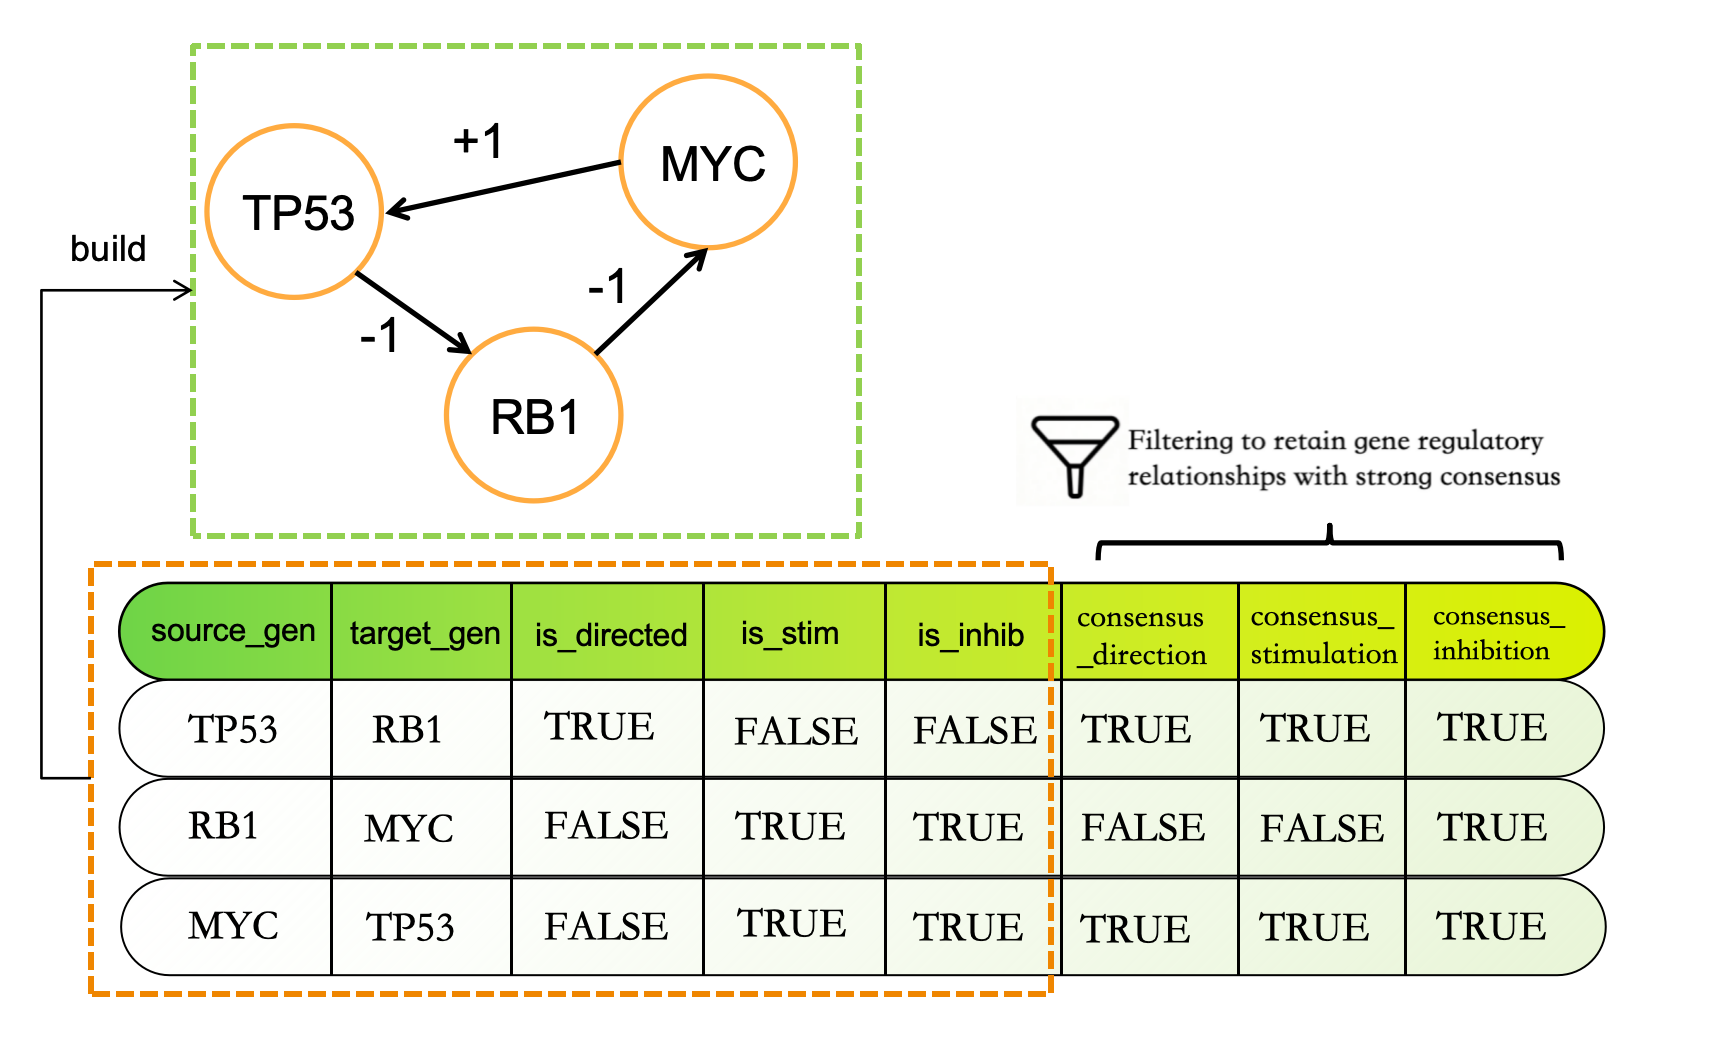
\includegraphics[width=0.95\linewidth]{figures/overview_of_omnipath.png}
    \caption[OmniPath Graph Construction]{Schematic overview of the OmniPath interaction tables and the graph construction used in this thesis. Each row in OmniPath describes a directed regulator to target relationship together with sign related fields (stimulation or inhibition) and consensus annotations. We filter to retain directed regulatory relationships with strong consensus and then convert the resulting edge list into a signed gene graph for downstream message passing.}
    \label{fig:overview_of_omnipath}
\end{figure}

\subsection{Summary}
\noindent After preprocessing, each modelling example contains a matched control expression profile $x_{\mathrm{ctl}}$, a treated expression profile used later to construct the response target together with the matched control, a drug feature vector aligned to the same gene order, and sample related identifiers such as cell line and profile ids. These inputs from each sample are combined with a fixed OmniPath derived interaction graph.

% \noindent Two gene spaces are supported. In landmark mode, the data use 978 genes and the aligned OmniPath graph contains 978 nodes and 1,627 directed edges. In the full gene setting, the data use 12,328 genes and the aligned OmniPath graph contains 12,328 nodes and 26,166 directed edges. In both settings, one gene order is used across control profiles, treatment profiles, response targets, drug feature vectors, and graph nodes.

